\chapter{Combinatorial Analysis}

\section{Why combinatorial analysis?}

A communication system consist of \(n\) seemingly identical antennas that are lined up in a linear ordered array. The resulting system will then be able to receive all incoming signals and will be called functional as long as no two consecutive antennas are defective. If \(m\) of the \(n\) antennas are defective, how many different states of the system are possible?

If \(n =4\) and \(m=2\) there are \(6\) states possible : 

\[ 
\begin{matrix}
    0 & 1 & 1 & 0 \\
    1 & 0 & 1 & 0 \\
    1 & 0 & 0 & 1 \\
    0 & 1 & 0 & 1 \\
    0 & 0 & 1 & 1 \\
    1 & 1 & 0 & 0 \\
\end{matrix}
\]

In \(6\) of these \(3\) of them are functional. 

\begin{definition}
    The mathematical theory of counting is known as \textbf{combinatorial analysis}  
\end{definition}

\section{The basic principle of counting}

\begin{definitionbox}[title=The Basic Principle of Counting]
    Suppose that two experiments are to be performed. The first experiment has \(m\) possible outcomes and for each of these outcomes the second experiment has \(n\) possible outcomes. Then the two experiments together have \(m \times n\) possible outcomes.
\end{definitionbox}
\begin{examplebox}[title=Example: Coin and Die]
    A coin is tossed and a die is rolled. How many possible outcomes are there?
    
    \textbf{Solution:} The coin has \(2\) possible outcomes and the die has \(6\) possible outcomes. Therefore the two experiments together have \(2 \times 6 = 12\) possible outcomes.
\end{examplebox}


\begin{definitionbox}[title=The Generalized Basic Principle of Counting]
    If \(r\) experiments are to be performed are to be such that the first one may result in any of \(n_1\) possible outcomes, and for each of these \(n_{1}\) possible outcomes there are \(n_2\) possible outcomes for the second experiment, and so on up to the \(r\)-th experiment which may result in any of \(n_r\) possible outcomes, then the \(r\) experiments together have \(n_1 \times n_2 \times \ldots \times n_r\) possible outcomes.
\end{definitionbox}


\begin{figure}[H]
    \centering
    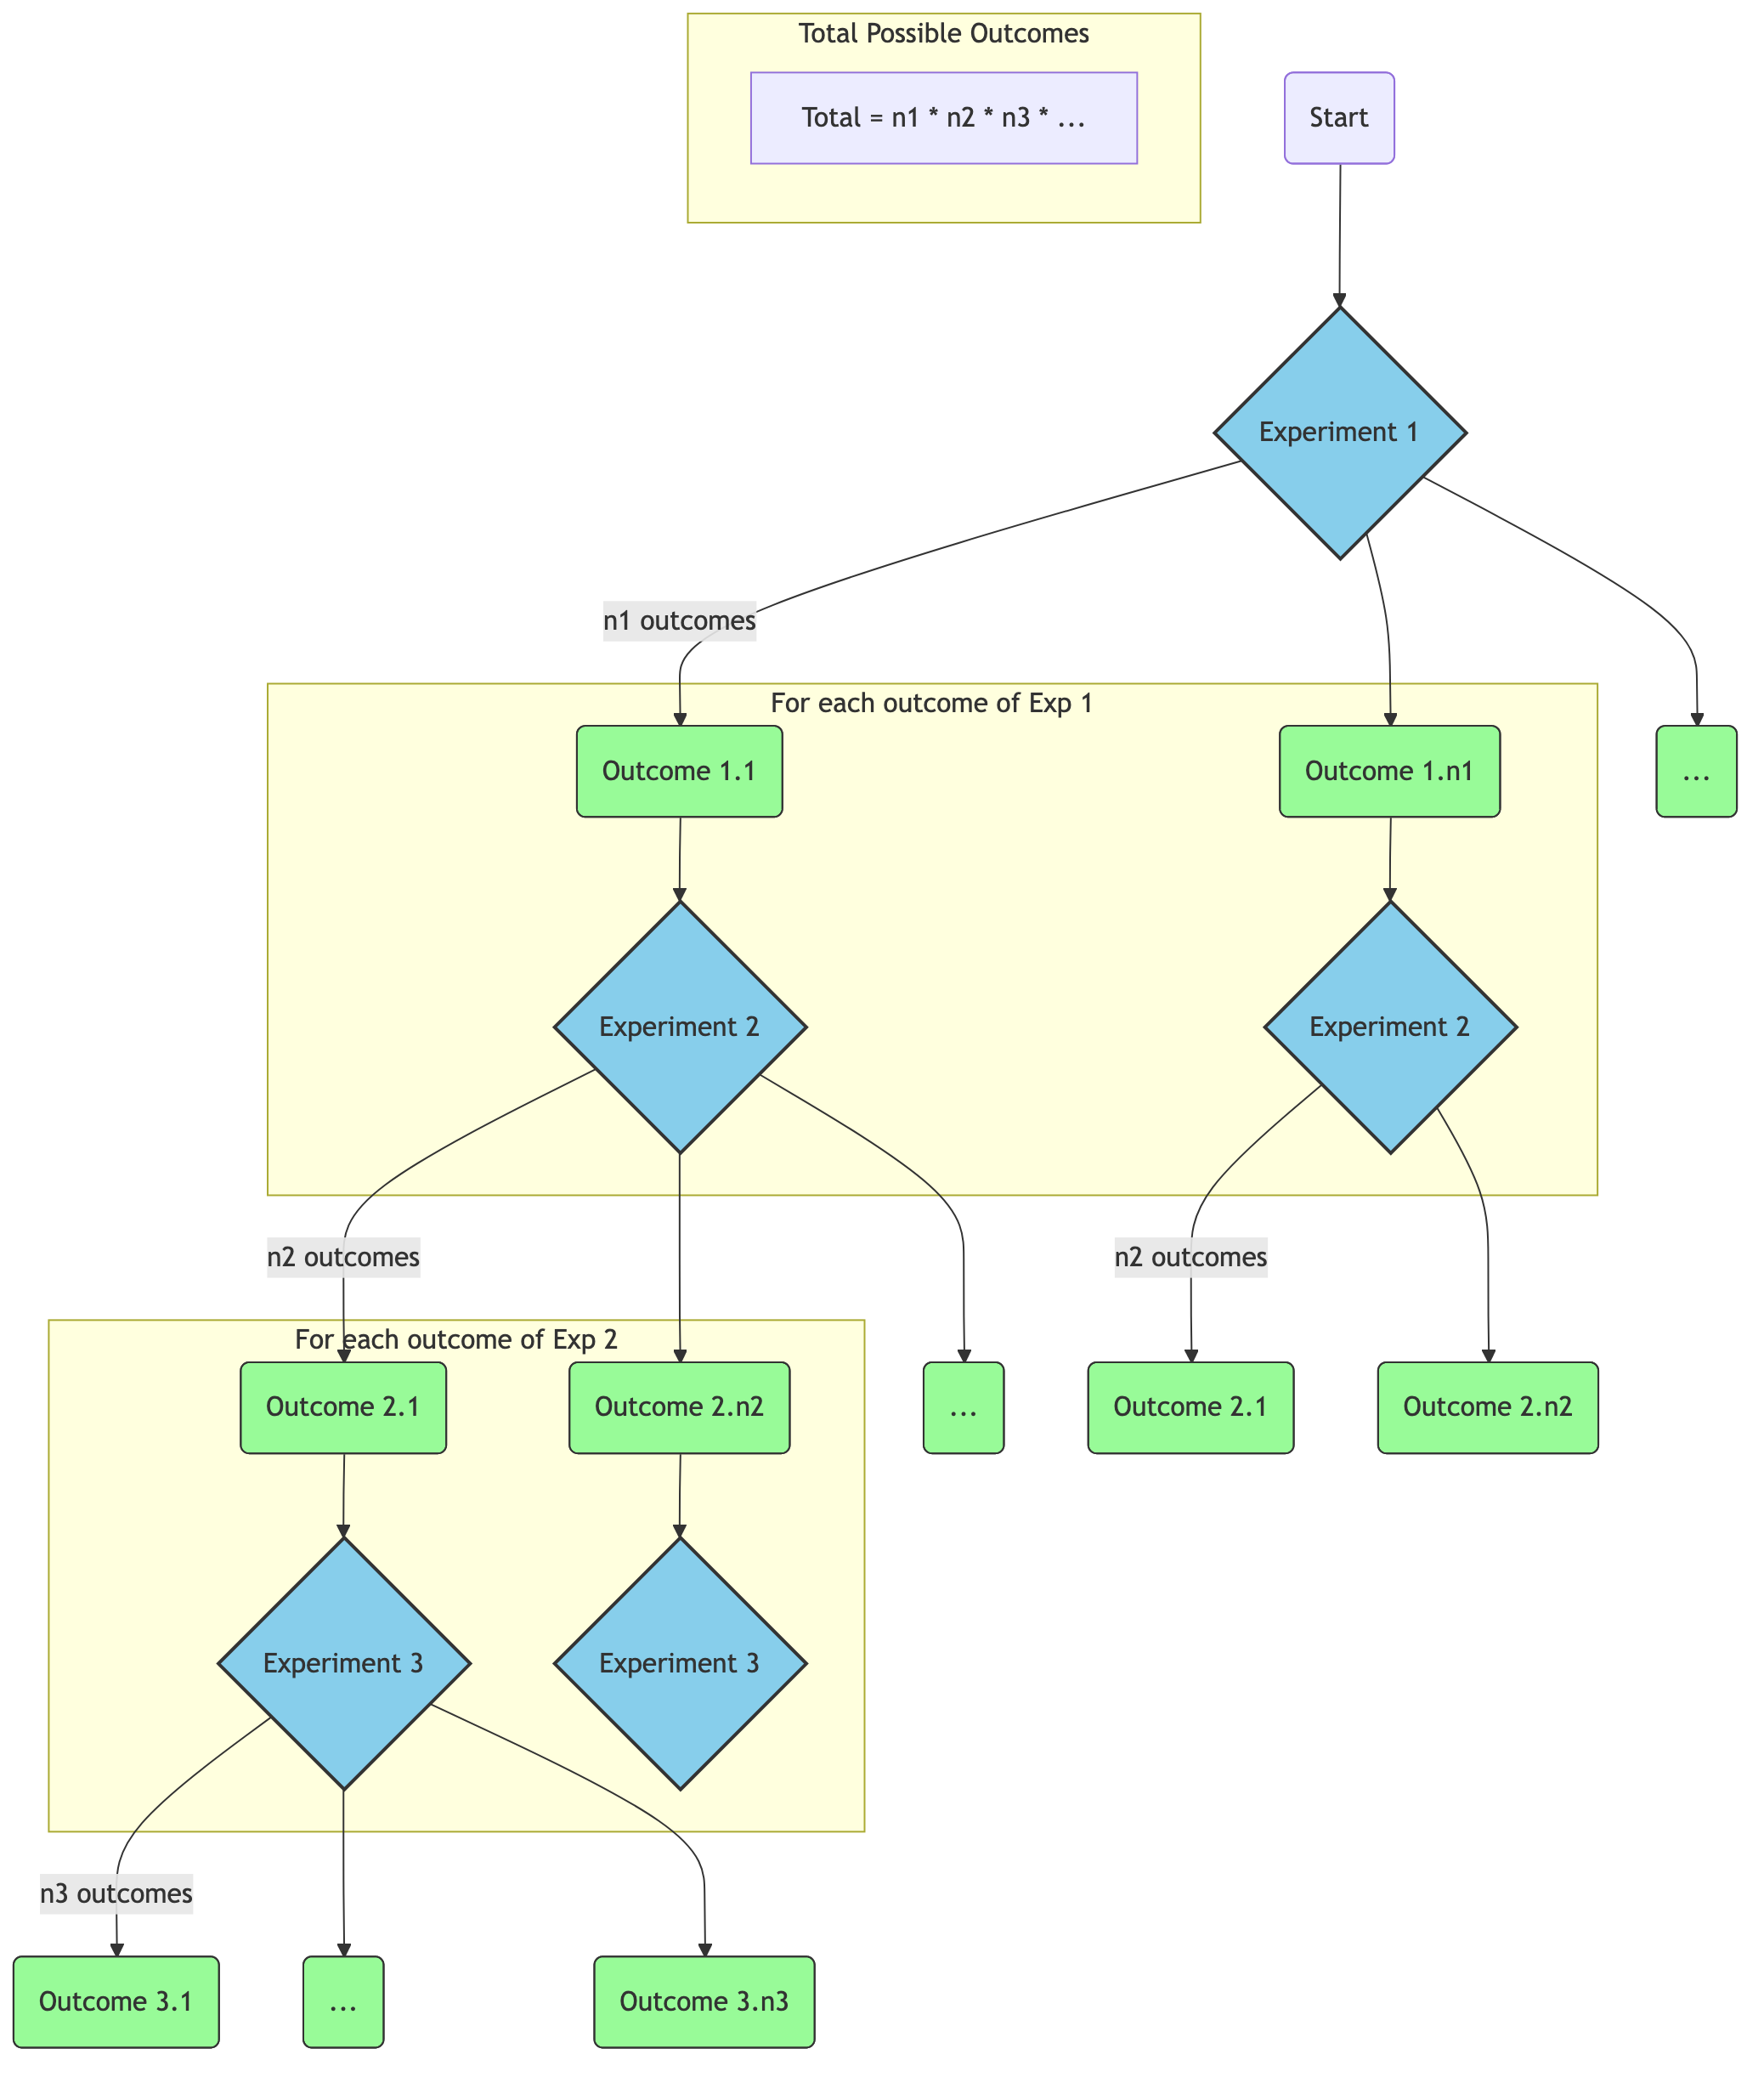
\includegraphics[width=0.8\textwidth]{counting.png}
    \caption{Mermaid diagram illustrating the Generalized Basic Principle of Counting}
    \label{fig:counting}
\end{figure}



\begin{examplebox}[title=Example: License Plates with Repetition]
    How many different \(7\) place license plates are possible if the first two places are to be occupied by letters and the remaining five by digits?
    
    \textbf{Solution:} The first two places can be filled with any of the \(26\) letters of the alphabet. Assuming letter can be repeated, the first place has \(26\) options and the second place has \(26\) options. The remaining five places can be filled with any of the \(10\) digits (from \(0\) to \(9\)), repeatedly. Therefore, the total number of different license plates is:

    \[
    26 \times 26 \times 10^5
    \]
\end{examplebox}

\begin{examplebox}[title=Example: License Plates without Repetition]
    If the letters and numbers in the previous example cannot be repeated, how many different license plates are possible?
    
    \textbf{Solution:} The first place has \(26\) options and the second place has \(25\) options (since letters cannot be repeated). The remaining five places can be filled with any of the \(10\) digits (from \(0\) to \(9\)). Therefore, the total number of different license plates is:

    \[
    26 \times 25 \times 10 \times 9 \times 8 \times 7 \times 6
    \]
\end{examplebox}

\section{Permutations}

\textbf{How many different ordered arrangements of letters \(a,b,c\) are possible?}

By enumeration we can see that : 

\[
abc, acb, bac, bca, cab, cba
\]
Each arrangement is called a \textbf{permutation} of the letters \(a,b,c\). There are \(6\) possible permutations for \(3\) distinct letters or a set of \(3\) distinct objects.

\begin{definitionbox}
    A permutation of \(n\) distinct objects is an arrangement of the objects in a specific order. The number of permutations of \(n\) distinct objects is given by \(n!\) (n factorial), which is the product of all positive integers up to \(n\):
    
    \[
    n! = n \times (n-1) \times (n-2) \times \ldots \times 2 \times 1
    \]
\end{definitionbox} 


\begin{examplebox}
    \textbf{Example 3:} How many different letter arrangments can be made from the letters PEPPER?
        \textbf{solution:} We have \(6\) letters in total where \(3\) letters are \(P\), \(2\) letters are \(E\) and \(1\) letter is \(R\). Therefore the number of different letter arrangements is given by:
        \[ \frac{6!}{3! \times 2! \times 1!} = 60 \]
        The idea is illustrated in Figure~\ref{fig:permute_pepper}.
\end{examplebox}

\begin{figure}[H!]
    \centering
    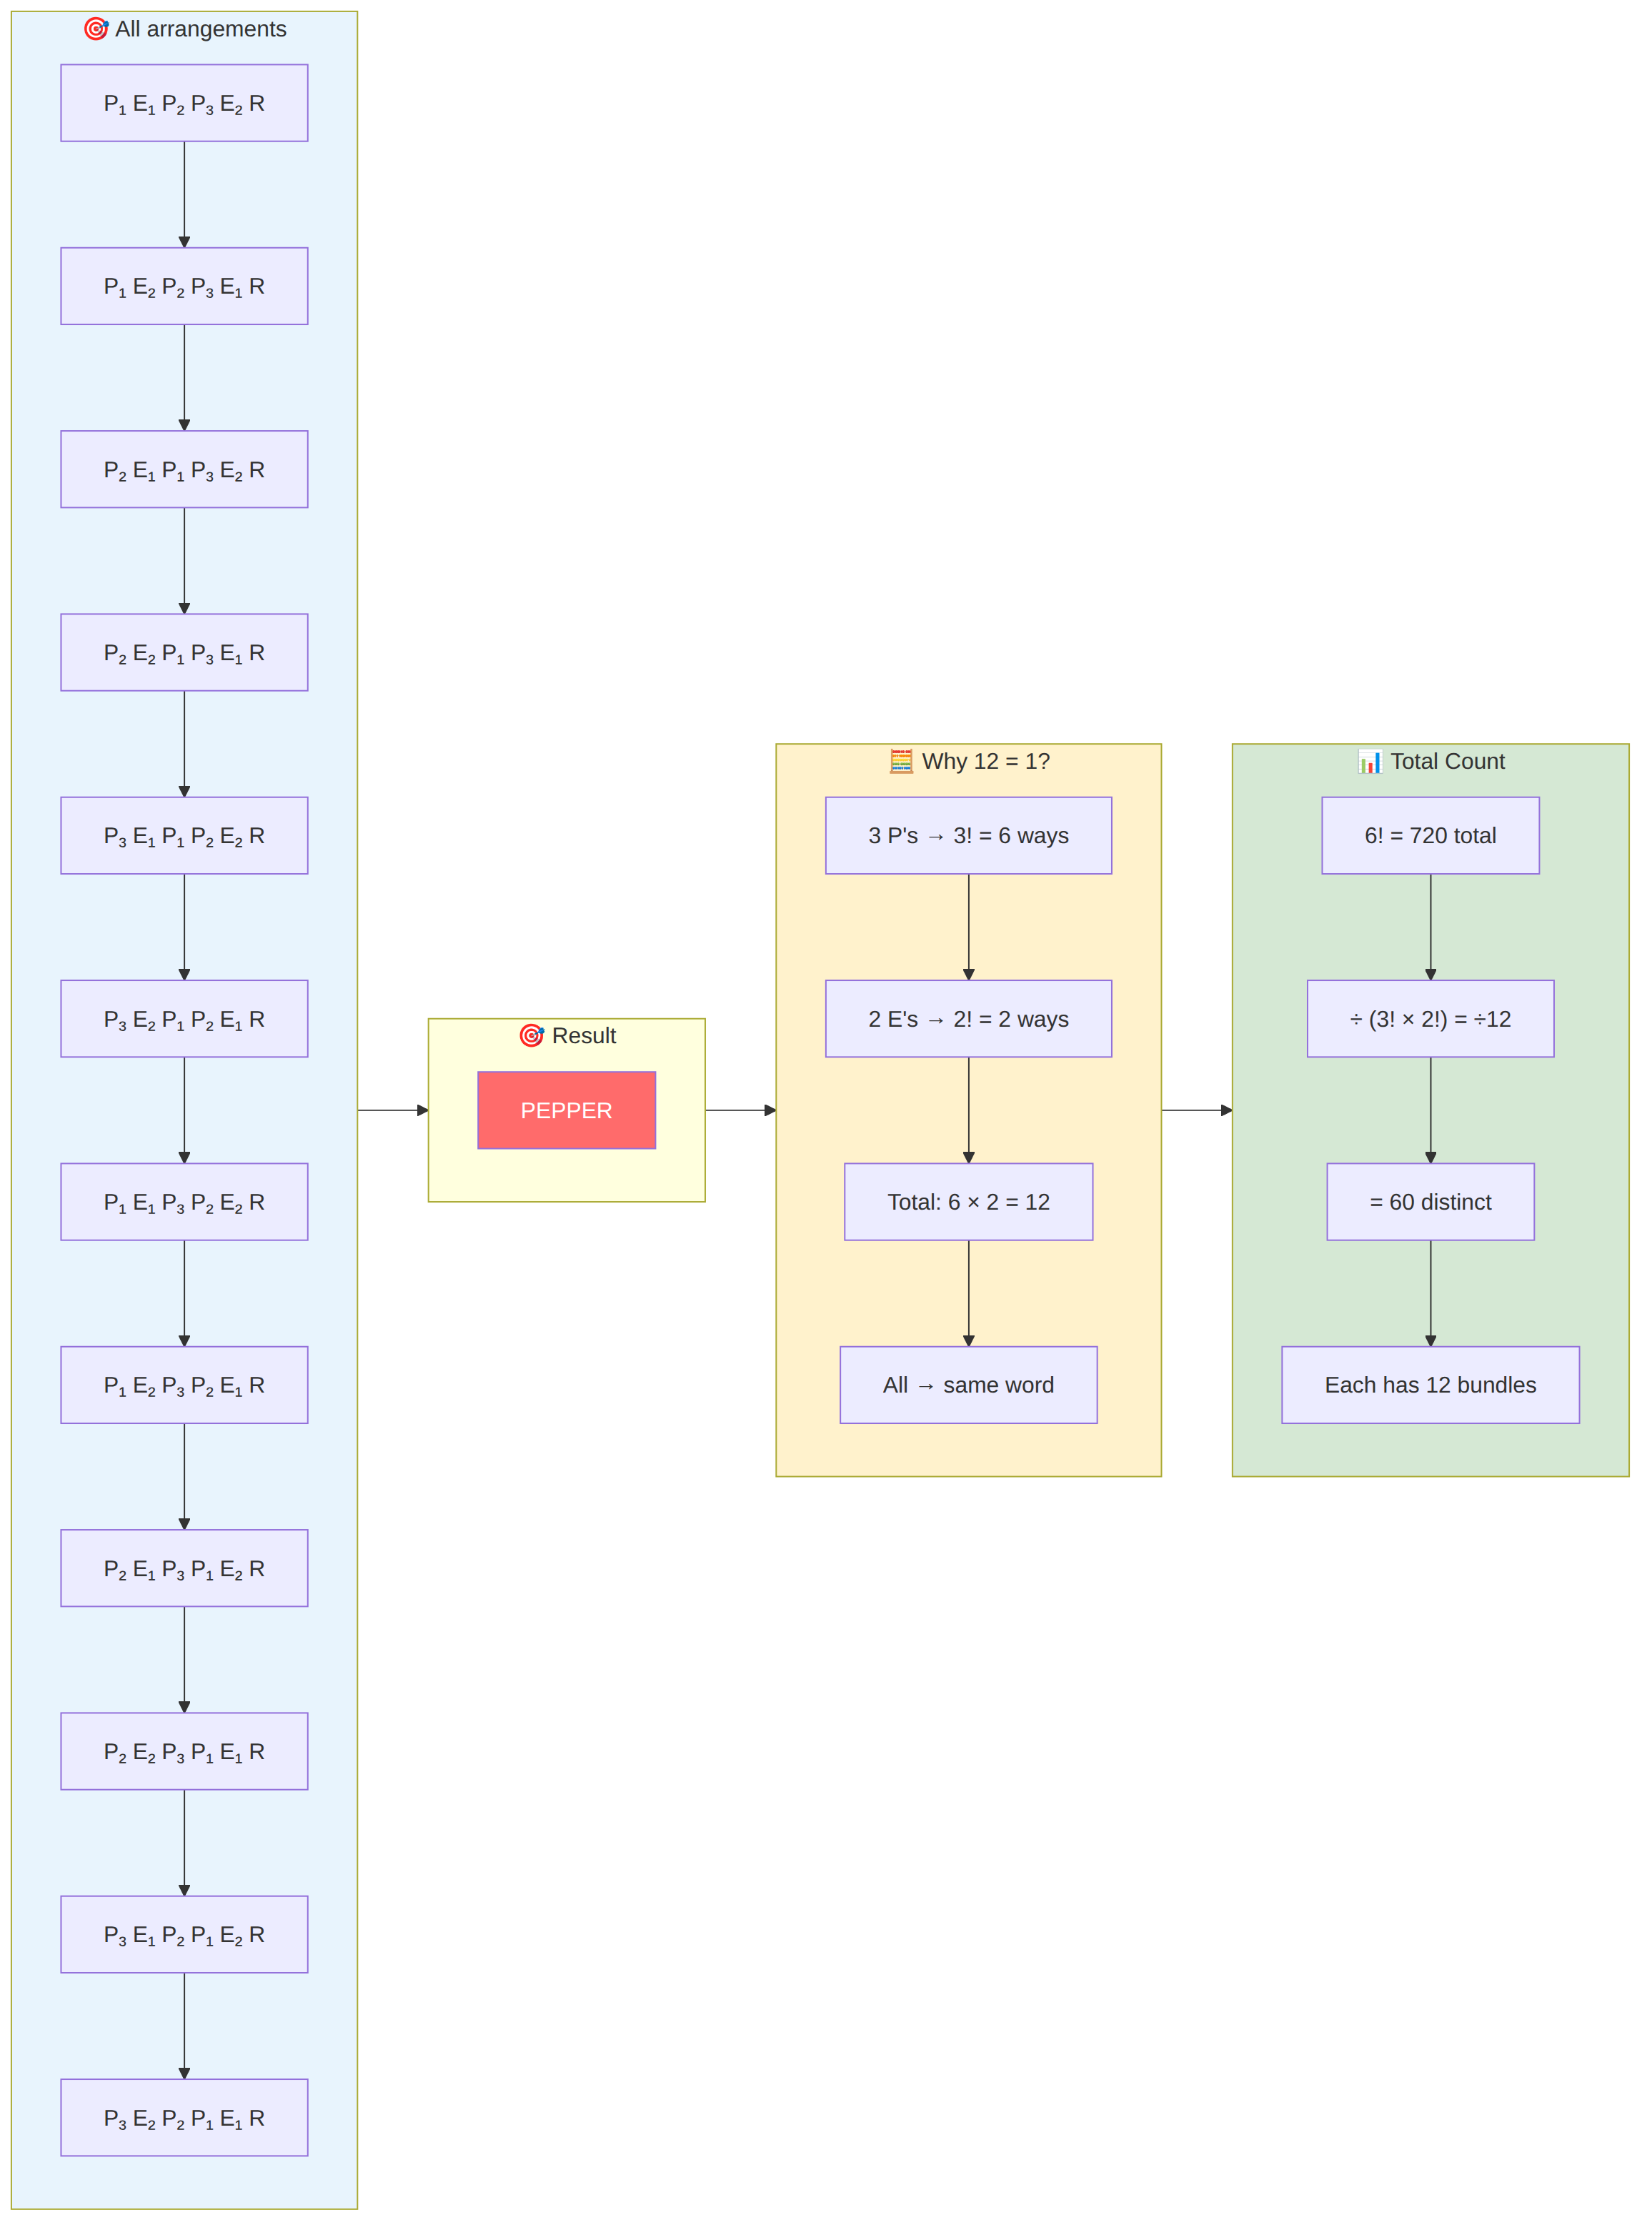
\includegraphics[width=1.1\textwidth]{permute_pepper_hd.png}
    \caption{The permutations of the letters in the word "PEPPER" by taking one permutation "PEPPER" and showing how many arrangements of the letters lead to the same word. This will repeat for other permutations as well}
    \label{fig:permute_pepper}
\end{figure}


\begin{keyconceptbox}{Permutations of k Objects from n Objects}
Let us start with \(n\) different objects and \(k\) be a positive integer such that \(k \leq n\). We want to determine the number of ways in which we can pick \(k\) objects from the total of \(n\) objects and arrange them in a sequence. i.e. the number of distinct \(k\) object sequence. We can do it in the following way 

\begin{itemize}
    \item We can pick the first object in \(n\) ways
    \item We can pick the second object in \(n-1\) ways (since we cannot pick the first object again)
    \item We can pick the third object in \(n-2\) ways (since we cannot pick the first and second objects again)
    \item ...
    \item We can pick the \(k\)-th object in \(n-(k-1)\) ways (since we cannot pick the first \(k-1\) objects again)
\end{itemize}

Therefore, by the generalized basic principle of counting, the total number of ways in which we can pick \(k\) objects from the total of \(n\) objects and arrange them in a sequence is given by
\[ 
    n \times (n-1) \times (n-2) \times \ldots \times (n-(k-1)) 
\]

\[
    = \frac{n(n-1)\cdots(n-(k-1))\times (n-k) \times (n-(k+1)) \times \cdots \times 2 \times 1}{(n-k) \times (n-(k+1)) \times \cdots \times 2 \times 1} 
\]

\[
= \frac{n!}{(n-k)!}
\]

In a special case when \(k=n\), we have
\[ \frac{n!}{(n-n)!} = \frac{n!}{0!} = n! \]
which is the number of ways in which we can arrange \(n\) distinct objects in a sequence.
\end{keyconceptbox}
\begin{exercisebox}
    \textbf{Exercise:} A chess tournament is to be held among \(10\) players. \(4\) are Russian, \(3\) are American, \(2\) are French and \(1\) is a German. How many different ways can the players be ranked from first to tenth place if the tournament just list the nationality of the players?
\end{exercisebox}


\begin{solutionbox}
    \textbf{Solution:} We have \(10\) players in total where \(4\) players are Russian, \(3\) players are American, \(2\) players are French and \(1\) player is German. Therefore the number of different ways the players can be ranked from first to tenth place is given by:
    \[ \frac{10!}{4! \times 3! \times 2! \times 1!} = 12600 \]
\end{solutionbox}

\section{Combinations}
\subsection{Inspiration}

Let's consider a problem: How many different groups of 3 objects could be formed from a total of 5 distinct objects A, B, C, D, and E?

If we think about selecting these objects in order, we'd have:
\begin{itemize}
    \item 5 ways to select the first object
    \item 4 ways to select the second object
    \item 3 ways to select the third object
\end{itemize}

Using the generalized basic principle of counting, we get $5 \times 4 \times 3 = 60$ ways of making ordered selections.

However, if we're only interested in which objects are in the group, not their order, then each distinct group is counted multiple times. For instance, the group \{A, B, C\} appears as all possible permutations: ABC, ACB, BAC, BCA, CAB, and CBA.

Since each group of 3 objects can be arranged in $3! = 6$ ways, the actual number of different groups is:
\[ \frac{5 \times 4 \times 3}{3!} = \frac{60}{6} = 10 \]

This illustrates the fundamental relationship between permutations and combinations: when we don't care about order, we divide the number of permutations by the number of ways to arrange the selected items.
\subsection{Definition}
\begin{definitionbox}
    A combination of \(n\) distinct objects taken \(r\) at a time is a selection of \(r\) objects from the total of \(n\) objects without regard to the order of selection. The number of combinations of \(n\) distinct objects taken \(r\) at a time is denoted by \(C(n,r)\) or \(\binom{n}{r}\) and is given by:
    
    \[
    C(n,r) = \binom{n}{r} = \frac{n!}{r!(n-r)!}
    \]
\end{definitionbox}

\begin{examplebox}[title=Example: Antennas with No Consecutive Defectives]
    \textbf{Problem:} Consider a set of $n$ antennas of which $m$ are defective and $n-m$ are functional. Assume that all defective antennas are indistinguishable from each other, and all functional antennas are indistinguishable from each other. How many linear orderings are there in which no two defective antennas are consecutive?
    
    \textbf{Solution:} This is a problem about combinations rather than permutations since we consider all defective antennas as identical, and likewise for functional antennas.
    
    To ensure no two defective antennas are consecutive, we need to place the $m$ defective antennas such that they are always separated by at least one functional antenna.
    
    Let's approach this by first placing the $n-m$ functional antennas in a row, creating $n-m+1$ potential positions for defective antennas (including before the first functional antenna, between functional antennas, and after the last functional antenna):
    
    \[
    \_ \circ \_ \circ \_ \circ \_ \cdots \circ \_
    \]
    
    where $\circ$ represents a functional antenna and $\_$ represents a potential position for defective antennas.
    
    Now, we need to choose $m$ positions out of these $n-m+1$ potential positions to place our defective antennas. This is a combination problem:
    
    \[
    \binom{n-m+1}{m} = \frac{(n-m+1)!}{m!(n-m+1-m)!} = \frac{(n-m+1)!}{m!(n-2m+1)!}
    \]
    
    Therefore, the number of linear orderings with no consecutive defective antennas is $\binom{n-m+1}{m}$.
    
    For example, if $n=7$ and $m=3$, then we have $\binom{7-3+1}{3} = \binom{5}{3} = 10$ possible arrangements with no consecutive defective antennas.
\end{examplebox}

\subsection{Pascal's Identity}
\begin{theorembox}[title=Pascal's Identity]
    For any integers \(n \geq 1\) and \(1 \leq k \leq n\),
    \[
    \binom{n}{k} = \binom{n-1}{k-1} + \binom{n-1}{k}
    \]
\end{theorembox}
\paragraph{Proof:}
We can prove Pascal's Identity using a combinatorial argument. Consider a set of \(n\) elements. We want to choose a subset of \(k\) elements from this set. We can do this in two ways:

1. **Case 1:** The first element is included in the subset. In this case, we need to choose \(k-1\) elements from the remaining \(n-1\) elements. The number of ways to do this is \(\binom{n-1}{k-1}\).

2. **Case 2:** The first element is not included in the subset. In this case, we need to choose \(k\) elements from the remaining \(n-1\) elements. The number of ways to do this is \(\binom{n-1}{k}\).

By considering both cases, we can express the total number of ways to choose \(k\) elements from \(n\) elements as the sum of the two cases:
\[
\binom{n}{k} = \binom{n-1}{k-1} + \binom{n-1}{k}
\]
This completes the proof of Pascal's Identity.

\subsubsection{Pascal's Triangle}
Pascal's Triangle is a triangular array of numbers where each number is the sum of the two directly above it. The \(n\)-th row corresponds to the coefficients in the expansion of \((x + y)^n\) and also represents the binomial coefficients \(\binom{n}{k}\).

\begin{figure}[h]
    \centering
    \begin{tabular}{ccccccccccc}
        & & & & & 1 & & & & & \\
        & & & & 1 & & 1 & & & & \\
        & & & 1 & & 2 & & 1 & & & \\
        & & 1 & & 3 & & 3 & & 1 & & \\
        & 1 & & 4 & & 6 & & 4 & & 1 & \\
        1 & & 5 & & 10 & & 10 & & 5 & & 1 \\
    \end{tabular}
    \caption{Pascal's Triangle showing the first 6 rows}
    \label{fig:pascal}
\end{figure}

\noindent
Each number in Pascal's Triangle is the sum of the two numbers above it. The value at position $(n,k)$ is $\binom{n}{k}$, where $n$ is the row number (starting from 0) and $k$ is the position within the row (also starting from 0).
\

\paragraph{The Connection:}
Pascal's Triangle is a direct visual representation of Pascal's Identity. The structure of the triangle is built using this identity as a fundamental rule. When constructing the triangle row by row, we start with 1 at the top and place 1's at both edges of each row (since $\binom{n}{0} = \binom{n}{n} = 1$). Every inner entry is then obtained by adding the two numbers directly above it—precisely following Pascal's Identity.

For example, examining row 4 ($n = 4$), the middle entry is $\binom{4}{2}$. By Pascal's Identity, this can be calculated as:
\[ \binom{4}{2} = \binom{3}{1} + \binom{3}{2} \]

Looking at the triangle, we can verify this: $3 + 3 = 6$, which is exactly the middle number in row 4. This pattern continues throughout the entire triangle, making it an elegant visual proof of Pascal's Identity and a useful tool for quickly calculating binomial coefficients.


\subsection{Binomial Theorm}
\begin{theorembox}[title=Binomial Theorem]
    For any integer \(n \geq 0\),
    \[
    (x + y)^n = \sum_{k=0}^{n} \binom{n}{k} x^{n-k} y^k
    \]
\end{theorembox}
\paragraph{Proof:}

\subsection{Binomial Theorem}
\begin{theorembox}[title=Binomial Theorem]
    For any positive integer \(n\),
    \[
    (x+y)^n = \sum_{k=0}^{n} \binom{n}{k} x^{n-k} y^k
    \]
\end{theorembox}
\paragraph{Proof:} Consider the product $(x+y)^n = \underbrace{(x+y)\,(x+y)\,\cdots\,(x+y)}_{\text{$n$ factors}}$.

When expanding this product, we must choose either $x$ or $y$ from each factor. To generate a term $x^{n-k}y^k$, we must select $y$ from exactly $k$ of the $n$ factors, and $x$ from the remaining $n-k$ factors.

The number of ways to select which $k$ factors contribute a $y$ is given by the binomial coefficient $\binom{n}{k}$. Thus, in the expansion, the coefficient of $x^{n-k}y^k$ is $\binom{n}{k}$.

Therefore:
\[
(x+y)^n = \sum_{k=0}^{n} \binom{n}{k}x^{n-k}y^k
\]

\begin{example}
For $n=3$:
\begin{itemize}[leftmargin=1.25em]
    \item $x^3$: choose $x$ from all factors (1 way)
    \item $x^2y$: choose $y$ from exactly 1 factor ($\binom{3}{1}=3$ ways)
    \item $xy^2$: choose $y$ from exactly 2 factors ($\binom{3}{2}=3$ ways)
    \item $y^3$: choose $y$ from all factors (1 way)
\end{itemize}

Thus $(x+y)^3 = x^3 + 3x^2y + 3xy^2 + y^3$, confirming the theorem.
\end{example}

\paragraph{Counting Principle Extension for Choosing Multiple Subsets}
We can extend our combinatorial principles to solve more complex problems, such as dividing a set into multiple groups. This directly connects to the concept of multinomial coefficients, which we'll explore next.

\subsection{Multinomial Coefficients}
\begin{definitionbox}[title=Multinomial Coefficient]
    Let $n$ and $r$ be positive integers, and let $n_1, n_2, \ldots, n_r$ be non-negative integers such that $n_1 + n_2 + \ldots + n_r = n$. The multinomial coefficient is defined as:
    \[
    \binom{n}{n_1, n_2, \ldots, n_r} = \frac{n!}{n_1! n_2! \cdots n_r!}
    \]
    
    This represents the number of ways to partition $n$ distinct objects into $r$ distinct groups, where group $i$ contains exactly $n_i$ objects.
\end{definitionbox}

\begin{examplebox}[title=Example: Committee Formation]
    A class of 20 students needs to form an executive committee with a president, vice president, secretary, and treasurer, and also needs to select 5 students for a planning committee and 6 students for a social committee. The remaining 5 students will not be on any committee. How many different ways can the committees be formed?
    
    \textbf{Solution:} This is a problem of partitioning 20 distinct students into 4 groups:
    \begin{itemize}
        \item 4 students for the executive committee
        \item 5 students for the planning committee
        \item 6 students for the social committee
        \item 5 students not on any committee
    \end{itemize}
    
    The number of ways to partition the students is:
    \[
    \binom{20}{4, 5, 6, 5} = \frac{20!}{4!5!6!5!} = 1,646,492,110,720
    \]
    
    However, within the executive committee, we must also assign specific roles. The 4 students can be arranged in $4! = 24$ ways. Therefore, the total number of different committee formations is:
    \[
    \frac{20!}{4!5!6!5!} \times 4! = \frac{20!}{5!6!5!} = 39,515,810,657,280
    \]
\end{examplebox}

\begin{examplebox}[title=Example: Division of Teams into Different Leagues]
        \textbf{Problem:} Ten children are to be divided into an A team and a B team of 5 each. The A team will play in one league and the B team in another. How many different divisions are possible?
        
        \textbf{Solution:} Since the teams are labeled (one specifically as "A team" for one league, the other as "B team" for another league), this is a case where we need to select which 5 children out of the 10 will be on the A team. The remaining 5 will automatically form the B team.
        
        The number of ways to select 5 children from 10 for the A team is given by:
        \[
        \binom{10}{5} = \frac{10!}{5!(10-5)!} = \frac{10!}{5!5!} = \frac{10 \times 9 \times 8 \times 7 \times 6}{5 \times 4 \times 3 \times 2 \times 1} = 252
        \]
        
        Therefore, there are 252 different possible divisions of the 10 children into the A and B teams.
\end{examplebox}

\begin{examplebox}[title=Example: Basketball Team Division]
    \textbf{Problem:} In order to play a game of basketball, 10 children at a playground divide themselves into two teams of 5 each. How many different divisions are possible?
    
    \textbf{Solution:} This problem requires us to determine whether the teams are considered distinguishable (labeled) or indistinguishable (unlabeled).
    
    Since we're forming teams for a basketball game with no specific designation (like "Team A" vs "Team B"), the teams are essentially unlabeled - swapping the two teams doesn't create a new division.
    
    If we were to choose which 5 children go into the first team, there would be $\binom{10}{5} = 252$ ways to do this. However, each division would be counted twice: once when a particular group of 5 is selected as the first team, and again when the complementary group of 5 is selected.
    
    Therefore, the number of different possible divisions is:
    \[
    \frac{1}{2}\binom{10}{5} = \frac{1}{2} \cdot 252 = 126
    \]
    
    There are 126 different ways to divide the 10 children into two teams of 5 each for the basketball game.
\end{examplebox}

\begin{keyconceptbox}{Labelled vs Unlabeled Teams}
The above problem illustrates the distinction between whether teams are considered \emph{labeled} or \emph{unlabeled}. Suppose we have $10$ children to be divided into two groups of $5$ each.

A fundamental problem in combinatorics involves partitioning a set into subsets, where the outcome depends critically on whether the subsets are considered \textbf{labeled} (distinguishable) or \textbf{unlabeled} (indistinguishable). Consider two scenarios: dividing ten children into a designated ``Team A'' and ``Team B'' of five each, or simply dividing them into two unnamed teams of five for a basketball game.

\medskip
\textbf{Case 1: Labeled teams (A team and B team).}  
Here the two groups are distinguished: one group is called the ``A team'' and the other is called the ``B team''. To form such a division, we only need to choose which $5$ children go into Team A, since the remaining automatically form Team B. The number of ways is
\begin{equation}
\binom{10}{5} \;=\; \frac{10!}{5!\,5!} \;=\; 252.
\end{equation}

\medskip
\textbf{Case 2: Unlabeled teams (pickup basketball game).}  
Here the two groups are indistinguishable: swapping the teams does not produce a new division. If we select any $5$ children as one side, we again obtain $\binom{10}{5} = 252$ possible choices. However, each division has been counted twice: once when a set of $5$ was chosen as ``Team 1,'' and again when its complement was chosen as ``Team 1.'' Therefore, the correct number of distinct (unordered) divisions is
\begin{equation}
\frac{1}{2}\binom{10}{5} \;=\; \frac{1}{2}\cdot 252 \;=\; 126.
\end{equation}

\medskip
\textbf{Small example check.}  
With $n=4$ children split into two groups of $2$, we have
\begin{align}
\text{Labeled teams: } & \binom{4}{2} = \frac{4!}{2!\,2!} = 6, \\
\text{Unlabeled teams: } & \frac{1}{2}\binom{4}{2} = \frac{6}{2} = 3.
\end{align}
Indeed, the three unique partitions are
\begin{equation}
\{AB \mid CD\}, \quad \{AC \mid BD\}, \quad \{AD \mid BC\}.
\end{equation}

\medskip
\textbf{Conclusion.}  
Hence, when dividing $10$ children into two teams of $5$:
\[
\text{Labeled teams (A vs. B)} \;\;\Rightarrow\;\; 252 \quad \text{divisions},
\]
\[
\text{Unlabeled teams (pickup game)} \;\;\Rightarrow\;\; 126 \quad \text{divisions}.
\]
The key insight is whether the symmetry of swapping teams is taken into account.

\end{keyconceptbox}


\begin{examplebox}
    In the first round of a knockout tournament involving $n = 2^m$ players, the $n$ players are divided into $n/2$ pairs, with each of these pairs then playing a game. The losers of the games are eliminated while the winners go on to the next round, where the process is repeated until only a single player remains. Suppose we have a knockout tournament of 8 players.

\begin{enumerate}[label=(\alph*)]
    \item How many possible outcomes are there for the initial round? (For instance, one outcome is that 1 beats 2, 3 beats 4, 5 beats 6, and 7 beats 8.)
    \item How many outcomes of the tournament are possible, where an outcome gives complete information for all rounds?
\end{enumerate}


\end{examplebox}

\begin{solutionbox}
    \textbf{(a) Possible Outcomes for the Initial Round}
To find the total number of outcomes for the first round, we must find the number of ways to pair the players and then multiply that by the number of possible results for those games.

\textbf{Step 1: Calculating the Number of Pairings}
We need to find the number of ways to divide 8 players into 4 unordered pairs.
\begin{itemize}
    \item The number of ways to choose the first pair is $\binom{8}{2}$.
    \item The number of ways to choose the second pair is $\binom{6}{2}$.
    \item The number of ways to choose the third pair is $\binom{4}{2}$.
    \item The number of ways to choose the final pair is $\binom{2}{2}$.
\end{itemize}
Since the order of the pairs does not matter that is (AB,CD,EF,GH) is same as (CD,AB,EF,GH), we must divide by $4!$, the number of ways to order the 4 pairs.
\begin{align*}
    \text{Number of Pairings} &= \frac{\binom{8}{2} \binom{6}{2} \binom{4}{2} \binom{2}{2}}{4!} \\
    &= \frac{\left(\frac{8 \times 7}{2}\right) \left(\frac{6 \times 5}{2}\right) \left(\frac{4 \times 3}{2}\right) \left(1\right)}{4 \times 3 \times 2 \times 1} \\
    &= \frac{28 \times 15 \times 6 \times 1}{24} \\
    &= \frac{2520}{24} = \mathbf{105}
\end{align*}
There are 105 unique ways to pair the 8 players.

\textbf{Step 2: Calculating the Game Results for Each Pairing}
For any given set of 4 pairs, there are 4 games. Each game has 2 possible outcomes (one player wins, the other loses).
\[
\text{Results per Pairing} = 2 \times 2 \times 2 \times 2 = 2^4 = \mathbf{16}
\]

\textbf{Step 3: Combining the Steps}
The total number of outcomes for the initial round is the product of the number of pairings and the number of results per pairing.
\[
\text{Total Outcomes (Round 1)} = 105 \times 16 = \mathbf{1680}
\]

\textbf{(b) Possible Outcomes for the Entire Tournament}

\textbf{The Elegant Method: A Permutation Approach}
A complete tournament outcome is uniquely determined by the sequence of eliminations. There is a one-to-one correspondence between every possible tournament outcome and every permutation of the $n$ players. For any given permutation of the 8 players, a unique tournament winner and history can be derived.

Therefore, the total number of possible outcomes is the number of permutations of 8 players, which is $8!$.
\begin{align*}
    \text{Total Outcomes} &= 8! \\
    &= 8 \times 7 \times 6 \times 5 \times 4 \times 3 \times 2 \times 1 \\
    &= \mathbf{40,320}
\end{align*}

\textbf{The Verification: A Round-by-Round Calculation}
We can verify this by multiplying the number of possible outcomes from each round.
\begin{itemize}
    \item \textbf{Round 1 (8 players $\to$ 4 winners):} From part (a), there are $\mathbf{1680}$ outcomes.
    
    \item \textbf{Round 2 (4 players $\to$ 2 winners):} 
    First, pair the 4 winners: $\frac{\binom{4}{2}\binom{2}{2}}{2!} = \frac{6 \times 1}{2} = 3$ ways.
    Next, for the 2 games, there are $2^2=4$ possible results.
    Total outcomes for this round: $3 \times 4 = \mathbf{12}$.
    
    \item \textbf{Round 3 (2 players $\to$ 1 winner):} 
    There is only 1 way to pair the final two players, and there are $2^1 = 2$ possible results.
    Total outcomes for this round: $1 \times 2 = \mathbf{2}$.
\end{itemize}
The total number of outcomes for the tournament is the product of the outcomes of each round:
\[
\text{Total Outcomes} = 1680 \times 12 \times 2 = \mathbf{40,320}
\]
Both methods yield the same result.
\end{solutionbox}

\begin{examplebox}
    Finding the number of integer solutions to an equation of the form
\[
x_1 + x_2 + \dots + x_k = n
\]
is a classic problem in combinatorics. The ``Stars and Bars'' method transforms this algebraic problem into a simple one of arranging objects.
\end{examplebox}

\begin{solutionbox}
    The analogy is as follows:
\begin{itemize}
    \item \textbf{Stars ($\star$):} The sum $n$ is treated as $n$ identical, indistinguishable items (stars).
    \item \textbf{Bins:} The $k$ variables ($x_1, \dots, x_k$) are treated as $k$ distinct bins. The value of a variable $x_i$ represents the number of stars in bin $i$.
    \item \textbf{Bars (|):} To separate the $k$ bins, we need exactly $k-1$ dividers (bars).
\end{itemize}
The problem then becomes: in how many ways can we arrange $n$ stars and $k-1$ bars?


\textbf{Case 1: Non-Negative Integer Solutions ($x_i \ge 0$)}
This is the most fundamental case where variables are allowed to be zero.

\textbf{Problem}
Find the number of integer solutions to $x_1 + x_2 + x_3 = 5$, where $x_1, x_2, x_3 \ge 0$.

\textbf{Solution Steps}
\begin{enumerate}
    \item \textbf{Identify $n$ and $k$:} We have $n=5$ (stars) and $k=3$ (bins).
    
    \item \textbf{Determine the number of bars:} To separate 3 bins, we need $k-1 = 2$ bars.
    
    \item \textbf{Frame the problem:} We need to find the number of unique arrangements of 5 stars and 2 bars. For example:
    \begin{itemize}
        \item \texttt{\star\star|\star|\star\star} corresponds to the solution $x_1=2, x_2=1, x_3=2$.
        \item \texttt{\star\star\star\star\star||} corresponds to the solution $x_1=5, x_2=0, x_3=0$.
        \item \texttt{|\star\star|\star\star\star} corresponds to the solution $x_1=0, x_2=2, x_3=3$.
    \end{itemize}
    
    \item \textbf{Calculate the arrangements:} We have a total of $n+k-1 = 5+3-1=7$ positions. We need to choose $k-1=2$ of these positions for the bars. This is a combination problem.
    \[
    \binom{n+k-1}{k-1} = \binom{7}{2} = \frac{7!}{2!(7-2)!} = \frac{7 \times 6}{2 \times 1} = \mathbf{21}
    \]
    There are 21 non-negative integer solutions.
\end{enumerate}

\textbf{General Formula ($x_i \ge 0$)}
The number of non-negative integer solutions to $x_1 + x_2 + \dots + x_k = n$ is:
\[
\binom{n+k-1}{k-1} \quad \text{or equivalently} \quad \binom{n+k-1}{n}
\]

\textbf{Case 2: Positive Integer Solutions ($x_i \ge 1$)}
A common variation where variables must be at least 1.
\textbf{Problem}
Find the number of integer solutions to $x_1 + x_2 + x_3 = 5$, where $x_1, x_2, x_3 \ge 1$.

\subsubsection*{Solution Steps}
\begin{enumerate}
    \item \textbf{The Strategy (Pre-distribution):} Since each variable must be at least 1, we first place one star in each of the $k=3$ bins. This uses up 3 stars. The number of stars remaining to be distributed is $n' = 5 - 3 = 2$.
    
    \item \textbf{Form a new equation:} The problem is now reduced to finding the number of non-negative solutions ($y_i \ge 0$) to a new equation with the remaining stars:
    \[
    y_1 + y_2 + y_3 = 2
    \]
    
    \item \textbf{Solve the new problem:} Using the formula from Case 1 with $n'=2$ and $k=3$:
    \[
    \binom{n'+k-1}{k-1} = \binom{2+3-1}{3-1} = \binom{4}{2} = \frac{4!}{2!2!} = \frac{4 \times 3}{2 \times 1} = \mathbf{6}
    \]
    There are 6 positive integer solutions.
\end{enumerate}

\textbf{General Formula ($x_i \ge 1$)}
The number of positive integer solutions is:
\[
\binom{n-1}{k-1}
\]

\textbf{Case 3: More Complex Constraints}
The method can be extended to any set of lower bounds by using a change of variables.

\textbf{Problem}
Find solutions for $x_1 + x_2 + x_3 = 12$, where $x_1 \ge 1, x_2 \ge 2, x_3 \ge 3$.

\textbf{Solution Steps}
\begin{enumerate}
    \item \textbf{The Strategy (Change of Variables):} Define new variables that are non-negative.
    \begin{align*}
        y_1 &= x_1 - 1 \ge 0 \\
        y_2 &= x_2 - 2 \ge 0 \\
        y_3 &= x_3 - 3 \ge 0
    \end{align*}
    This is equivalent to pre-distributing 1 star to bin 1, 2 to bin 2, and 3 to bin 3.
    
    \item \textbf{Substitute into the equation:} Rewrite the original equation in terms of the new variables.
    \begin{align*}
        (y_1+1) + (y_2+2) + (y_3+3) &= 12 \\
        y_1 + y_2 + y_3 + 6 &= 12 \\
        y_1 + y_2 + y_3 &= 6
    \end{align*}
    
    \item \textbf{Solve the standard problem:} We now find the non-negative solutions for this new equation, with $n=6$ and $k=3$.
    \[
    \binom{n+k-1}{k-1} = \binom{6+3-1}{3-1} = \binom{8}{2} = \frac{8 \times 7}{2 \times 1} = \mathbf{28}
    \]
    There are 28 solutions that meet the specified conditions.
\end{enumerate}
\end{solutionbox}









\section{Applications of Combinatorial Analysis}
Combinatorial analysis has applications in various fields, including computer science, statistics, and operations research. Some common applications include:
\begin{itemize}
    \item Cryptography: Designing secure communication systems. For example, in RSA encryption, large prime numbers are used to create keys where the security relies on the computational difficulty of finding the prime factorization of large numbers.
    
    \item Network Design: Optimizing the layout of networks. For instance, determining the minimum number of routers needed to connect all computers in an office while minimizing cable length is a combinatorial optimization problem.
    
    \item Game Theory: Analyzing strategies in competitive situations. For example, in poker, calculating the probability of certain card combinations helps players make optimal betting decisions based on possible opponent hands.
    
    \item Probability Theory: Calculating probabilities in complex scenarios. For instance, in quality control, determining the probability of finding defective items in a batch using sampling techniques relies on combinatorial calculations.
\end{itemize}
